\documentclass{article}
\usepackage{pdfpages}
\usepackage{booktabs}
\usepackage{pdfpages}

\begin{document}
\section*{Summary}
This is a book, containing the results summarized from the Light curve simulated data from Alex, shown in figure(\ref{A}). Here we have used $3$ filters from the data. The original time delay and magnification in the data is found in the title of the plot. We tried with changing the node spacing in the recontruction process. So an array of node spacing prior range was chosen and for each of this value, the reconstruction was done and the results are compared, which can be seen in the table in next page. The posterior plots and the reconstructed images for each of this rows from the table are subsequently presented in the following pages in the same order as of the rows in the table's node-space values.
Changing the upper range of the time delay maximum range, can however change the reconstruction and the fitting statistics. The upper range of this parameter which is called as 'dt\_max'in the program, used in this run of the code, can be found in the naming nomenclature of the folder TD\_$30$, meaning the uppper range of the time delay max is $30$ day (the default lower limit is $0$). The folder name also shows the number of parameter used which is $NP=8$. 
  
%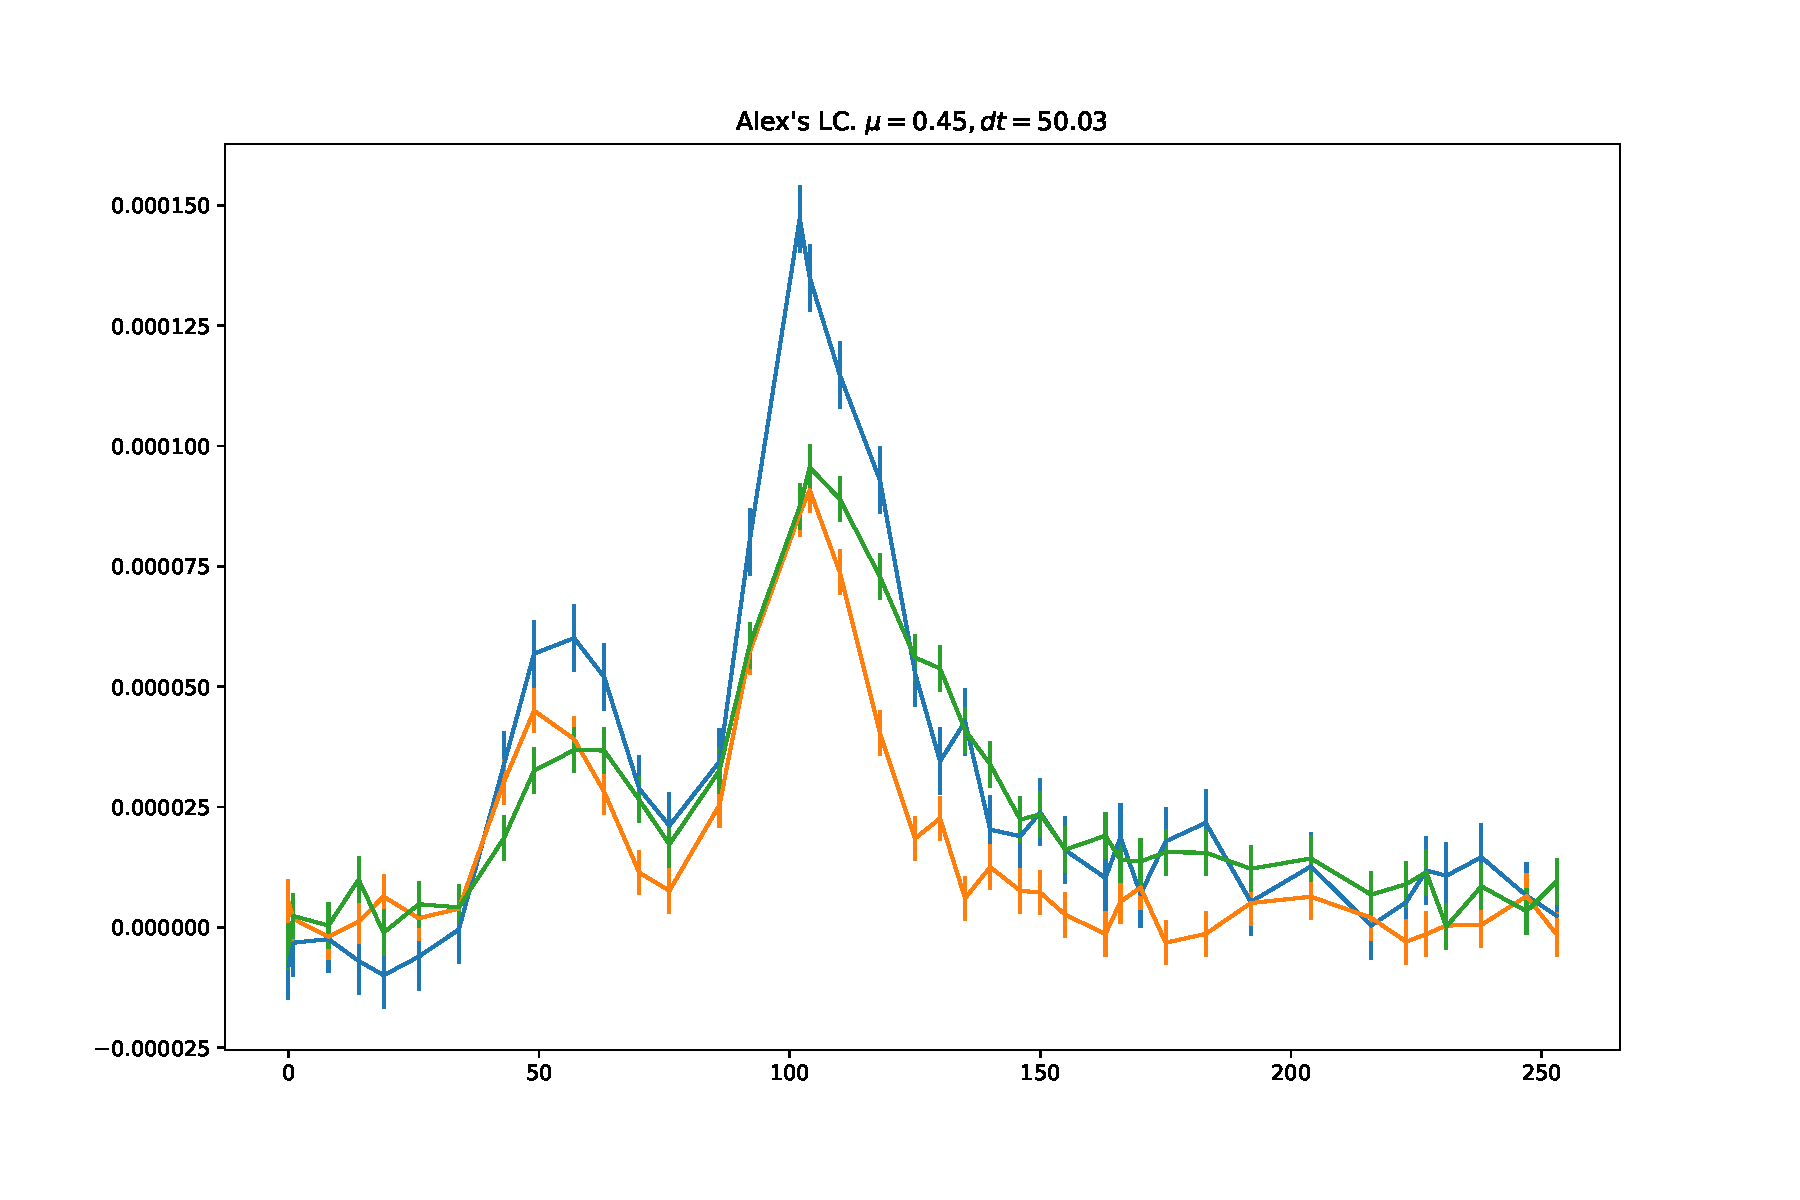
\includepdf[pages=-]{Alex_LC.pdf}\label{A}

\begin{figure}[h!]
  \centering
    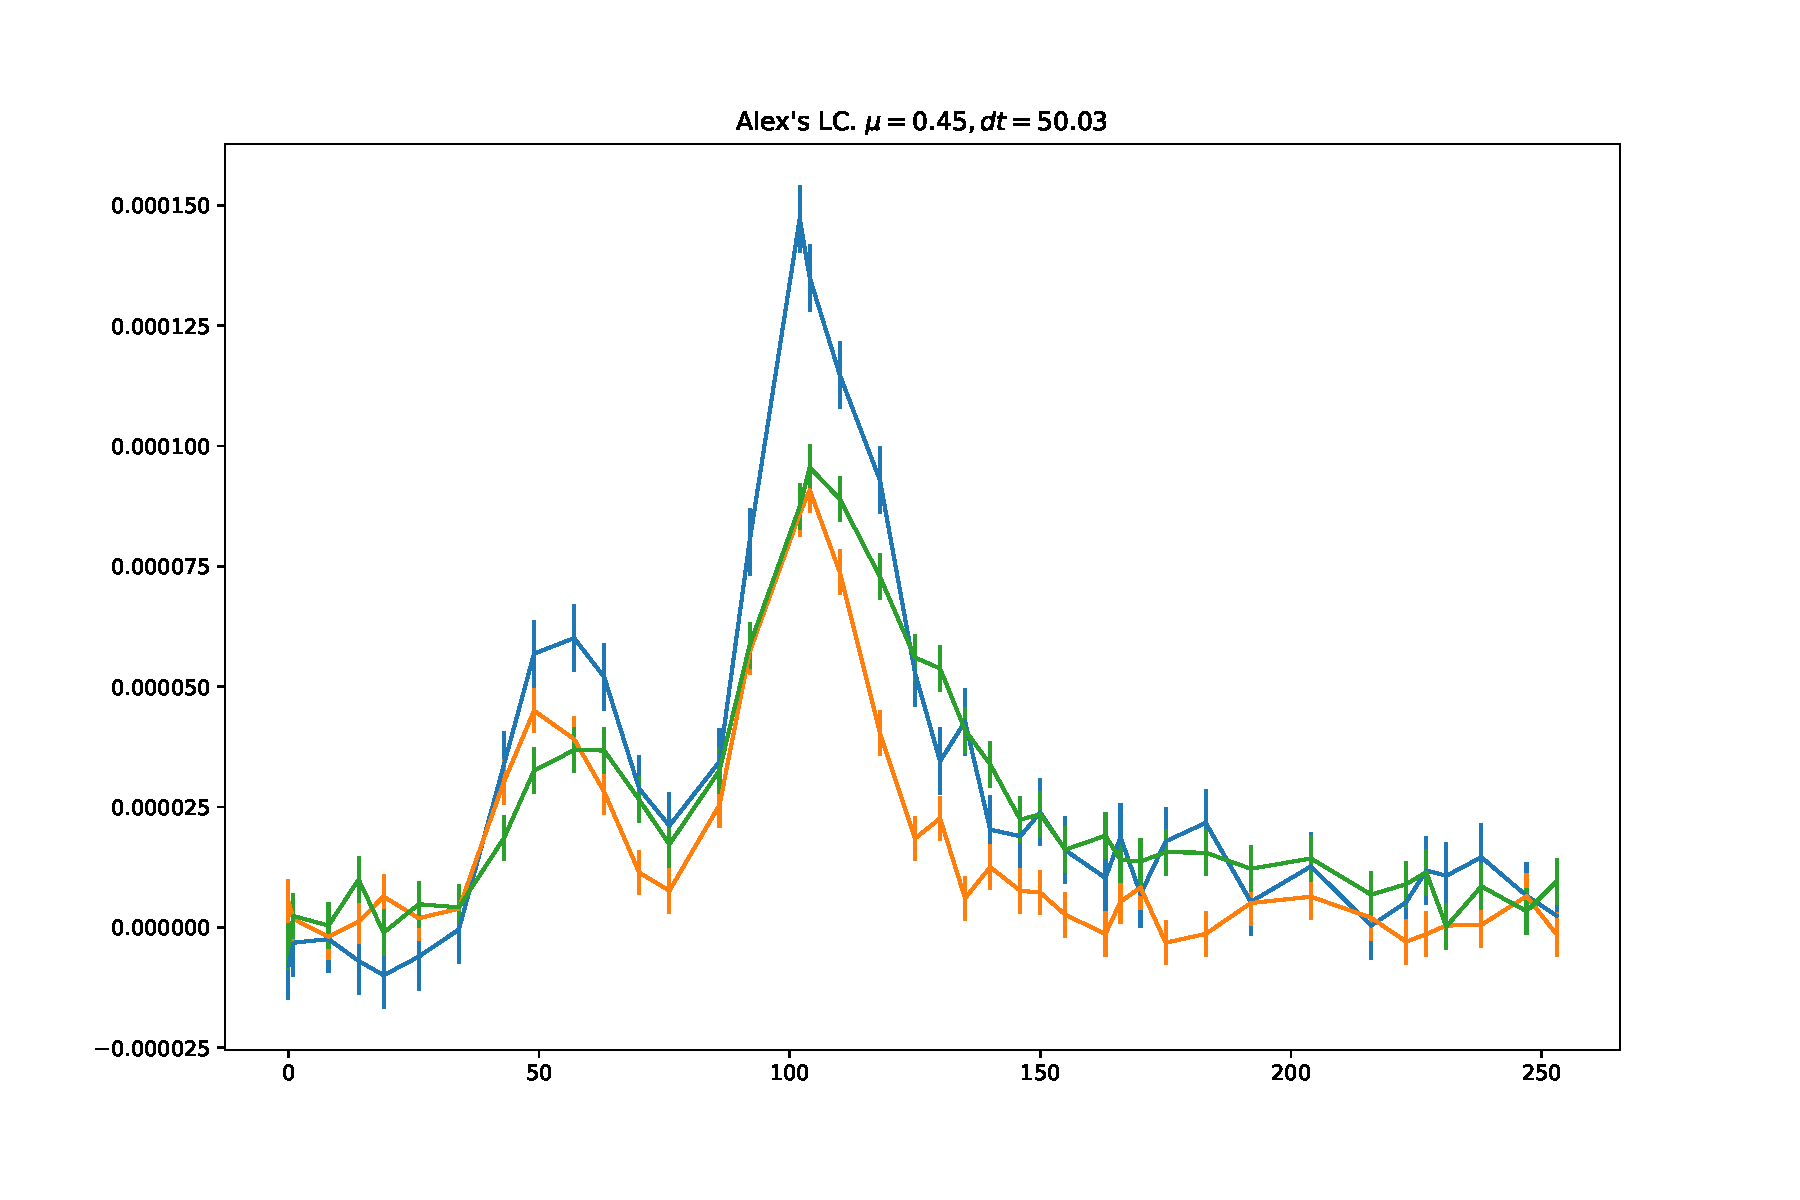
\includegraphics[width=\textwidth]{Alex_LC.pdf}
  \caption{Alex's simulated light curve, customised to produce $2$ images, with a time delay and magnification(ralative) shown in the top header of the plot. Here we used only $3$ filter data, which are shown above.\\\hspace{\textwidth}\textbf{X-axis = Time Delay in Days, Y-Axis = Flux.}}
  \label{A}
\end{figure}


\iffalse
\begin{tabular}{|r|r|r|r|r|r|r|r|}
\toprule
 nspace &  mu\_expec &  dt\_expec &    mu\_pos &     dt\_pos &      chi\_r &       chi\_g &      chi\_i \\
\midrule
    0.2 &  0.447761 &   50.0321 &  0.992106 &  16.186471 &  80.095808 &  131.032903 &  68.984341 \\
    0.8 &  0.447761 &   50.0321 &  0.993098 &  16.170706 &  80.133262 &  131.150938 &  68.961759 \\
    0.9 &  0.447761 &   50.0321 &  0.993060 &  16.177268 &  80.110177 &  131.132301 &  68.949017 \\
    1.0 &  0.447761 &   50.0321 &  0.993052 &  16.181014 &  80.123145 &  131.090523 &  68.989736 \\
    3.0 &  0.447761 &   50.0321 &  0.991982 &  16.175313 &  80.133453 &  131.119943 &  68.928404 \\
   10.0 &  0.447761 &   50.0321 &  0.993098 &  16.183023 &  80.157793 &  131.061535 &  69.015544 \\
   30.0 &  0.447761 &   50.0321 &  0.991972 &  16.182894 &  80.148067 &  131.073688 &  68.990985 \\
   30.0 &  0.447761 &   50.0321 &  0.991889 &  16.168123 &  80.105236 &  131.213501 &  68.872679 \\
   60.0 &  0.447761 &   50.0321 &  0.991908 &  16.179790 &  80.131513 &  131.078189 &  68.960297 \\
\bottomrule
\end{tabular}
\fi
\iffalse

\fi
Table in the next page, showing the reconstruction statistics, \textbf{as a function of the node space parameter($1^{st}$ column)} for a given dt\_max(which in this case is $30$ for $NP=8$ parameters.
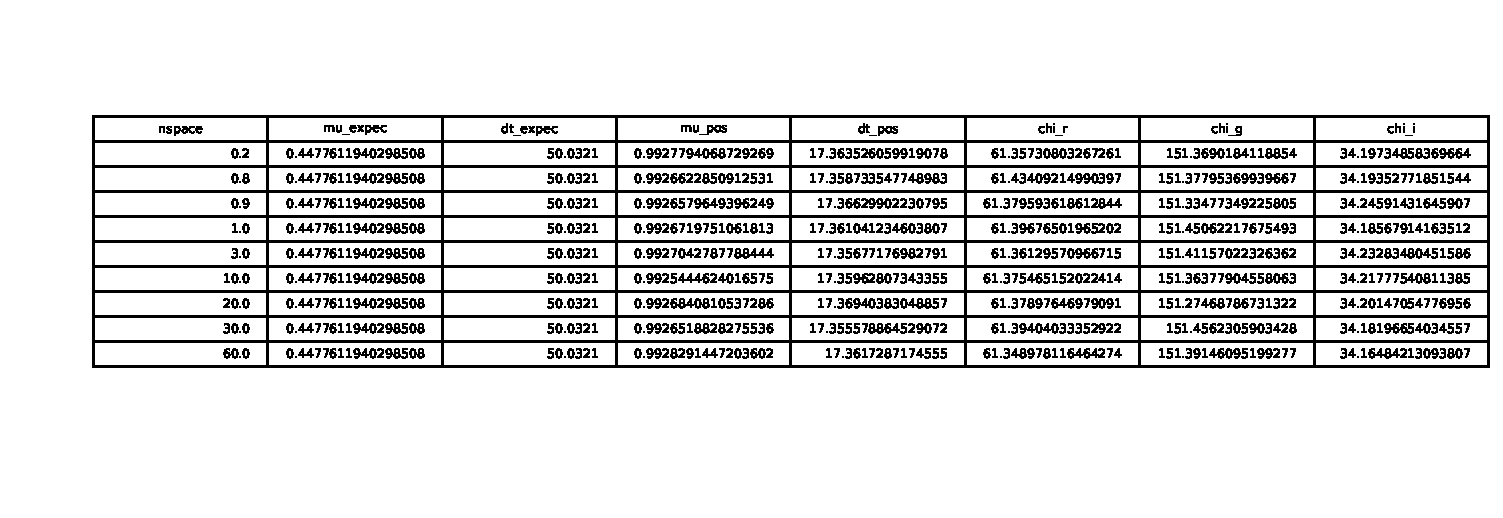
\includepdf[pages=-]{Reconstruction-TD_30_NP_8.pdf}\label{T}

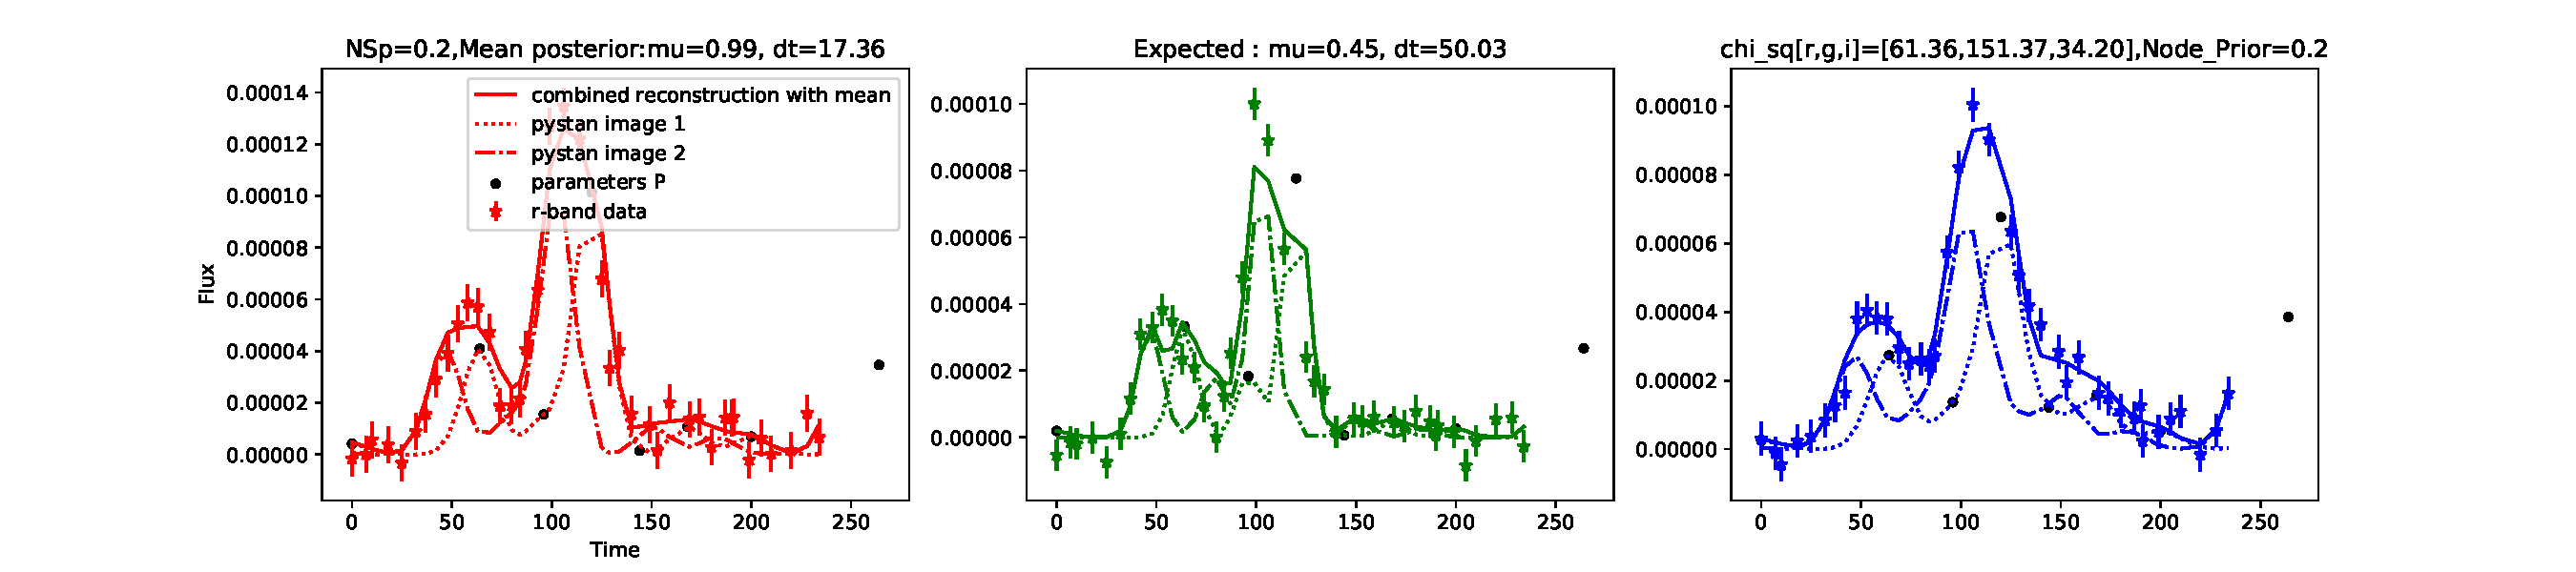
\includepdf[pages={1-},nup=1x4,scale=1.0]{Reconstruction-TD_30_NP_8_plots.pdf}

%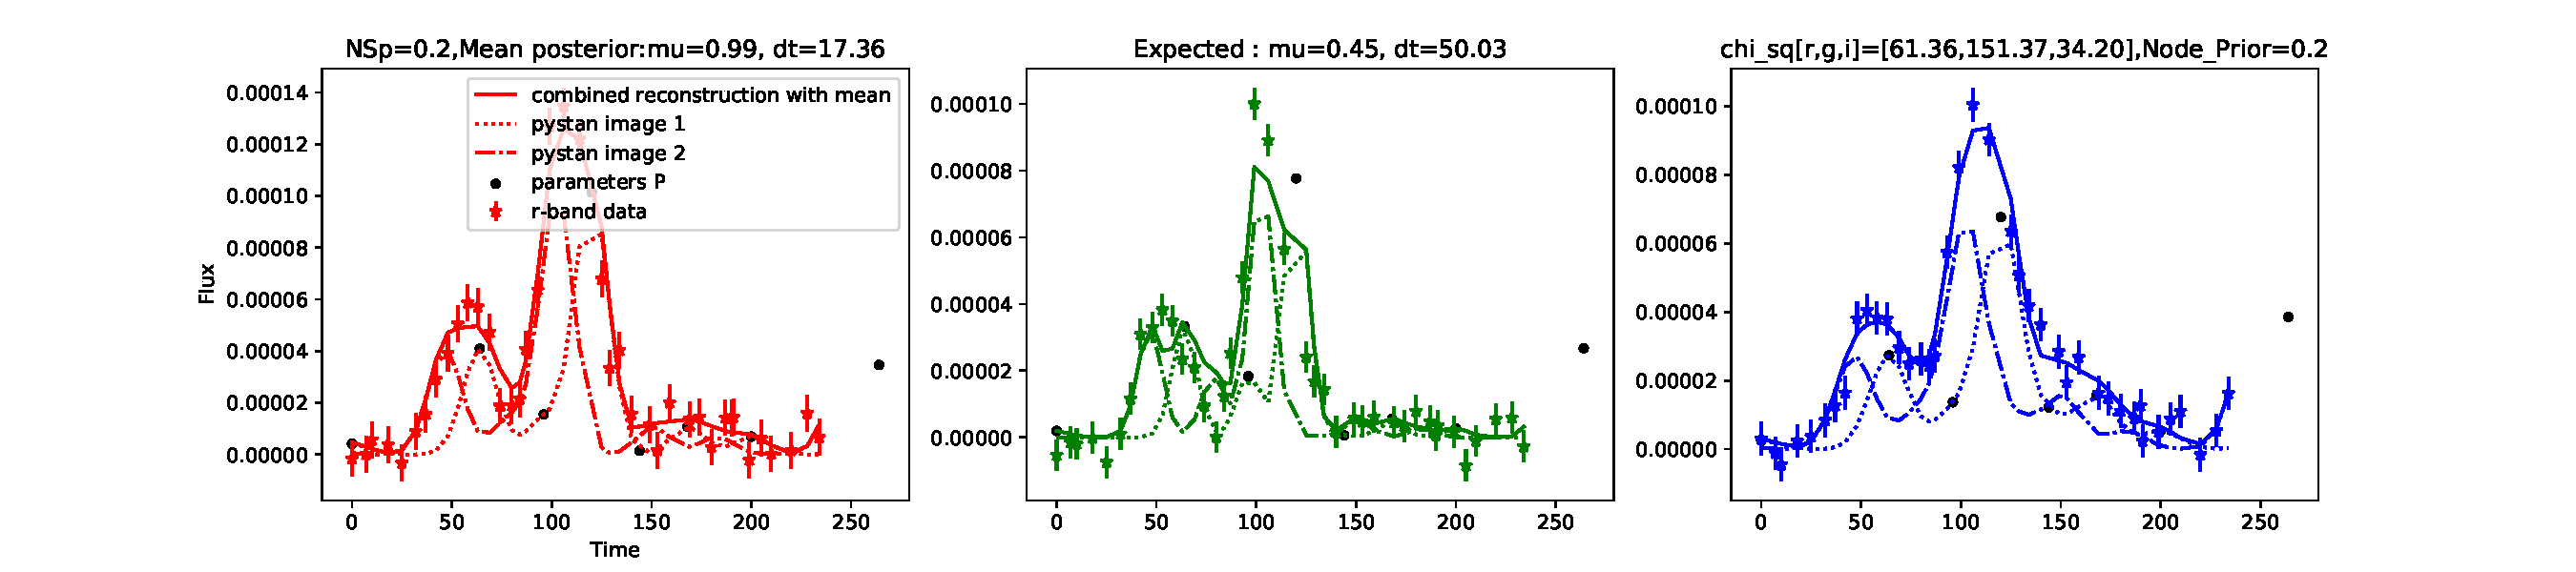
\includepdf[pages=-]{Reconstruction-TD_30_NP_8_plots.pdf}
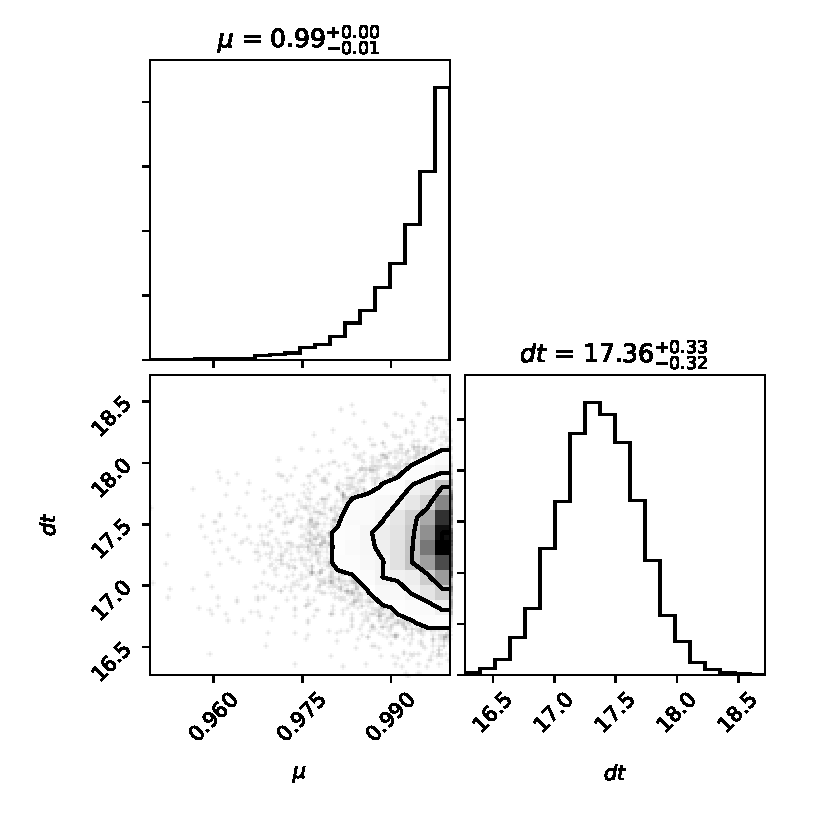
\includepdf[pages={1-},nup=2x2,scale=1.0]{corner-TD_30_NP_8.pdf}
%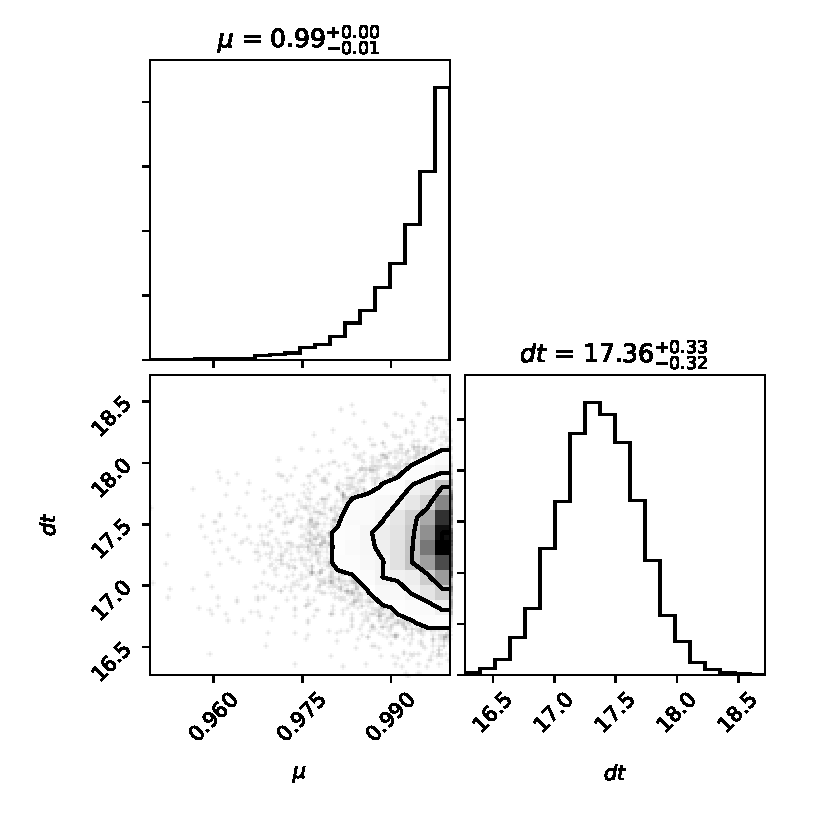
\includepdf[pages=-]{corner-TD_30_NP_8.pdf}
\end{document}
